\longnewglossaryentry{gls-MVM}{name=Motion Movement file}{See \ref{mvm-file} MVM files}

\newacronym[see={[Glossary:]{gls-MVM}}]{MVM}{MVM}{Motion Movement file (inaccurate)\glsadd{gls-MVM}}

\longnewglossaryentry{gls-STL}{name=Stereo Lithography Files}{STL files describe the surface geometry of a three-dimensional object without any representation of color, texture or other common CAD model attributes. An STL file describes a raw unstructured triangulated surface by the unit normal and vertices of the triangles using a three-dimensional Cartesian coordinate system. STL coordinates must be positive numbers, there is no scale information, and the units are arbitrary \cite{stl-wikipedia}.	
	The STL format specifies both ASCII and binary representations. Binary files are more common, since they are more compact.\newline
	In the \emph{Jaw Viewer}, each STL-File represents one \gls{mesh} or one \gls{anatomy}.
}

\newacronym[see={[Glossary:]{gls-STL}}]{STL}{STL}{Stereo Lithography Files\glsadd{gls-STL}}


\longnewglossaryentry{mesh}{name=Mesh, plural=Meshes}{A mesh is a software abstraction (a class) used for the graphical representation of coordinate collections or \gls{vertex} and can be static or animated. In the \emph{Jaw Viewer}, a mesh represents an \gls{anatomy}. Each Mesh class instance has the logic which allow rendering itself.
}

\longnewglossaryentry{anatomy}{name=Anatomy Object}{Is the real physical object corresponding to a \gls{mesh}, is a body part, in this context a jaw bone. Its description is contained in \gls{STL} files and its software abstraction is a \gls{mesh}. 
	\begin{figure}[h!]
		\centering
		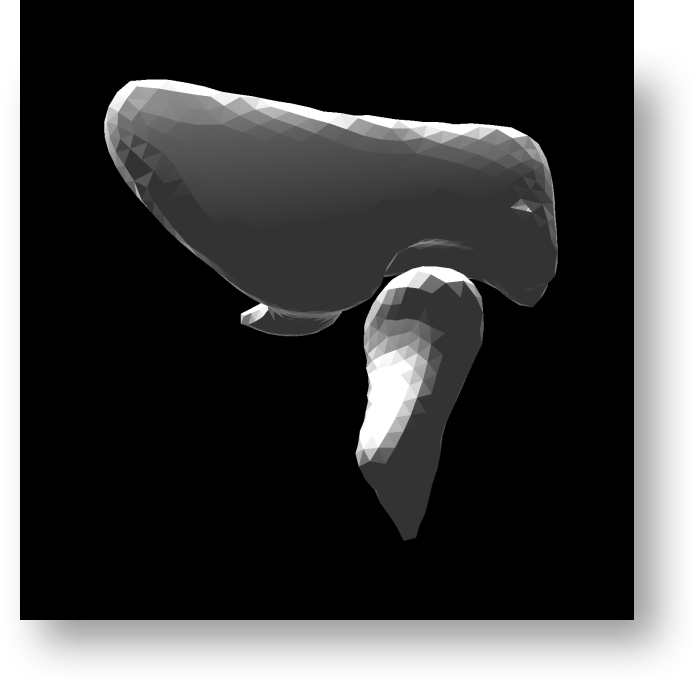
\includegraphics[width=0.35\textwidth]{anatomy}
		\label{fig:stl}
		\caption{A Mesh, STL File or Anatomy Object}
	\end{figure}
}


\longnewglossaryentry{sphere}{name=Reference Sphere}{Reference Sphere}

\longnewglossaryentry{calibration}{name=Calibration Data}{Calibration data from the Zeiss Cameras}

\longnewglossaryentry{opengl}{name=OpenGL}{OpenGL \cite{openglweb} is the premier environment for developing portable, interactive 2D and 3D graphics applications. Since its introduction in 1992, OpenGL has become the industry's most widely used and supported 2D and 3D graphics application programming interface (API), bringing thousands of applications to a wide variety of computer platforms. OpenGL fosters innovation and speeds application development by incorporating a broad set of rendering, texture mapping, special effects, and other powerful visualization functions. Developers can leverage the power of OpenGL across all popular desktop and workstation platforms, ensuring wide application deployment.}


\longnewglossaryentry{vertex}{name=Vertex,plural=Vertices}{A point in space is both a vertex and a vector \cite{superbible}. Except when used for point and line \glspl{primitive}, it also defines the point at which two edges of a polygon meet.
	\begin{figure}[h!]
		\centering
		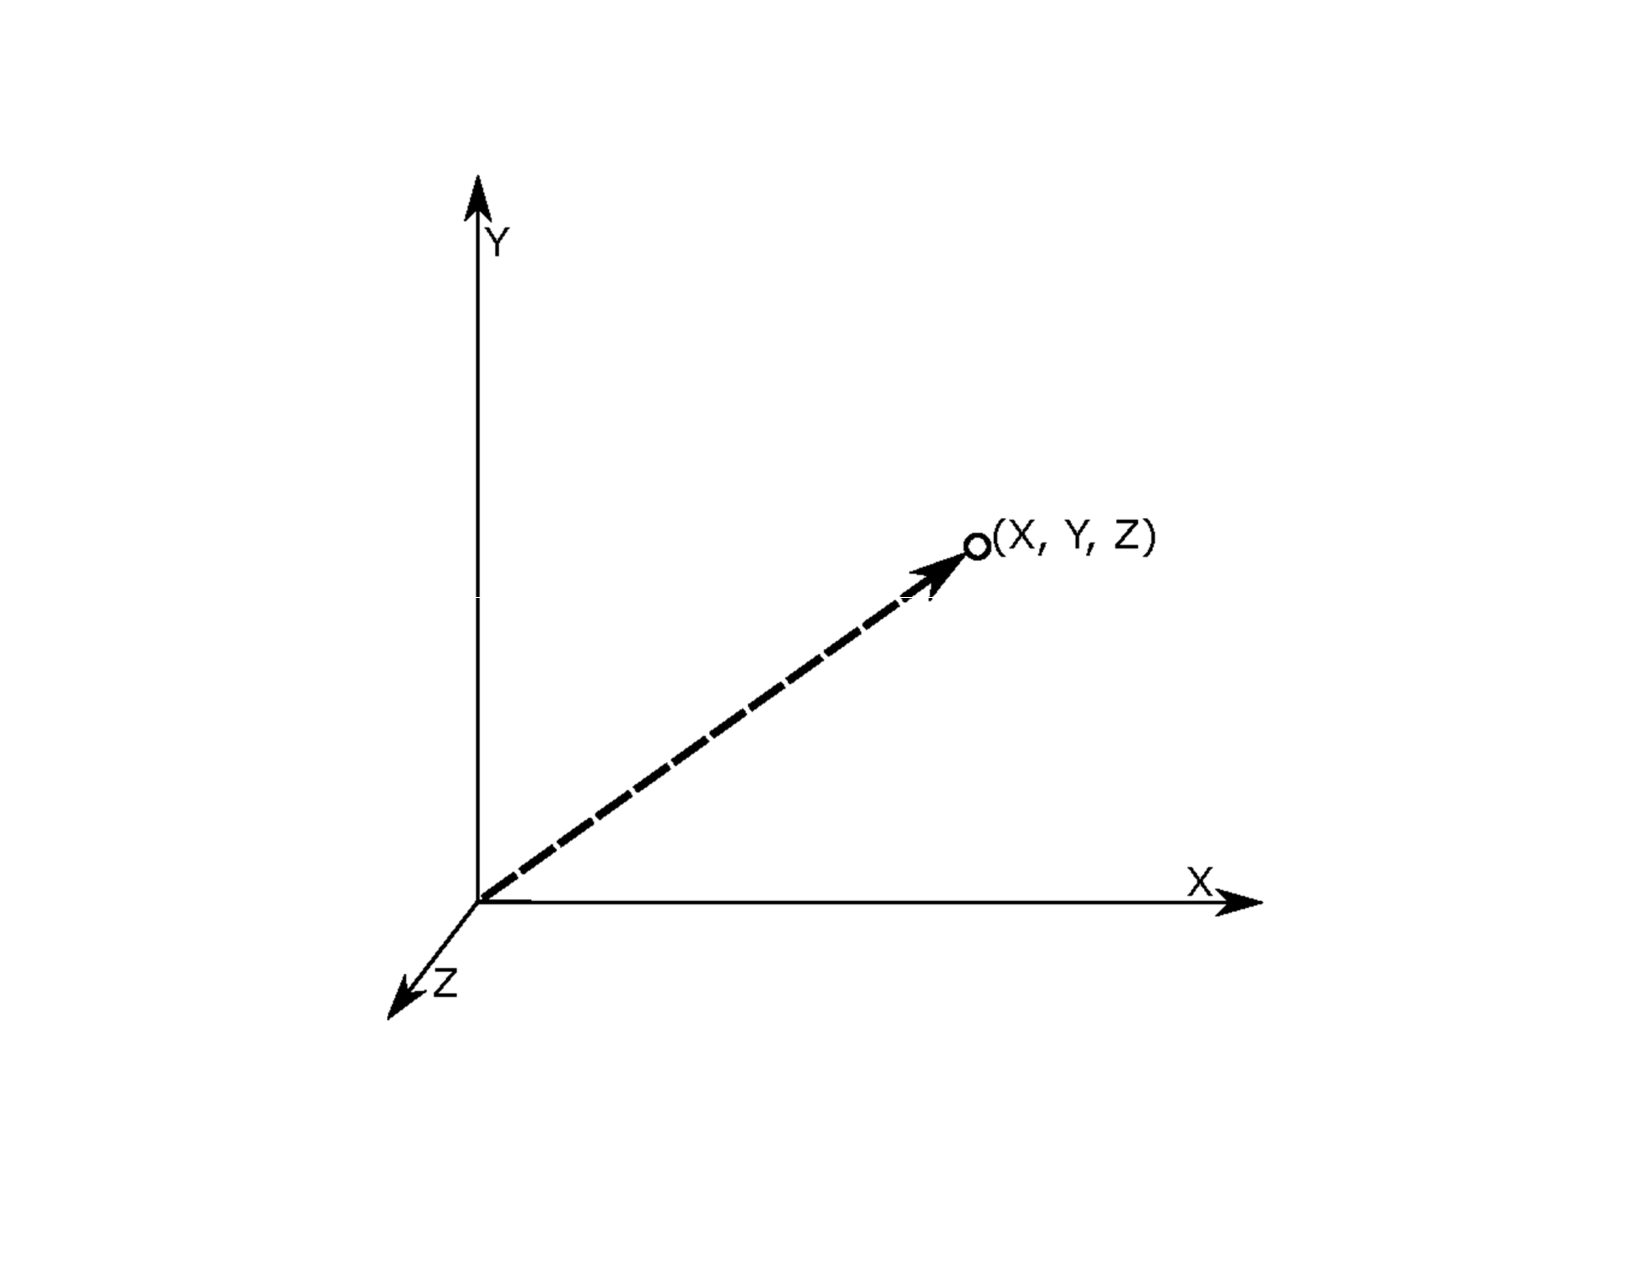
\includegraphics[width=0.25\textwidth]{vertex}
		\label{fig:vertex}
		\caption{Vertex \cite{superbible}}
	\end{figure}
}

\longnewglossaryentry{primitive}{name=Primitive,plural=primitives}{A group \cite{superbible} of one or more \glspl{vertex} formed by OpenGL into a geometric shape such as a line, point, or triangle. All objects and scenes are composed of various combinations of primitives. Everything you see rendered on the screen is a collection of primitives.}

\longnewglossaryentry{model-view-matrix}{name=Model-view matrix}{The OpenGL matrix that transforms position vectors from model (or object) space to view (or eye) space.\cite{superbible}}

\longnewglossaryentry{perspective}{name=Perspective}{A drawing mode in which objects farther from the viewer appear smaller than nearby objects.\cite{superbible}}

\longnewglossaryentry{vertex-shader}{name=Vertex shader}{A \gls{shader} that executes once per incoming vertex. \cite{superbible} }

\longnewglossaryentry{viewport}{name=Viewport}{The area within a window that is used to display an \gls{opengl} image. Usually, this encompasses the entire client area. Stretched viewports can produce enlarged or shrunken output within the physical window. \cite{superbible} }

\longnewglossaryentry{fragment-shader}{name=Fragment shader}{A \gls{shader} that executes once per fragment and generally computes the final color of that fragment.\cite{superbible}}

\longnewglossaryentry{geometry-shader}{name=Geometry shader}{A \gls{shader} that executes once per primitive, having access to all vertices making up that primitive.\cite{superbible}}

\longnewglossaryentry{shader}{name=Shader}{A small program that is executed by the graphics hardware, often in parallel, to operate on individual \glspl{vertex} or pixels \cite{superbible}. There are \glspl{vertex-shader}, \glspl{fragment-shader} and \glspl{geometry-shader}}

\longnewglossaryentry{gls-normalized-device-coordinates}{name=Normalized Device Coordinates}{The \gls{NDC} \cite{learnopengl} are in a small space where $x, y$ and $z$ values vary from $-1.0$ to $1.0$. Any coordinates that fall outside this range will be discarded/clipped and won't be visible on your screen. Below you can see the triangle we specified within normalized device coordinates (ignoring the $z$ axis): 
		\begin{figure}[h!]
		\centering
		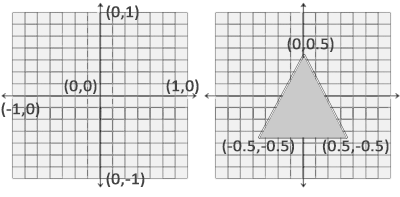
\includegraphics[width=0.3\textwidth]{ndc}
		\label{fig:ndc}
		\caption{Normalized Device Coordinates \cite{learnopengl}}
	\end{figure} 
Unlike usual screen coordinates the positive y-axis points in the up-direction and the $(0,0)$ coordinates are at the center of the graph, instead of top-left. Eventually you want all the (transformed) coordinates to end up in this coordinate space, otherwise they won't be visible. }

\newacronym[see={[Glossary:]{gls-normalized-device-coordinates}}]{NDC}{NDC}{Normalized Device Coordinates\glsadd{gls-normalized-device-coordinates}}

\longnewglossaryentry{model-space}{name=Model Space}{Positions relative to a local origin. Also sometimes known as \emph{\gls{object-space}}. \cite{superbible}}

\longnewglossaryentry{object-space}{name=Object Space}{Positions relative to a local origin. Also sometimes known as \emph{\gls{model-space}}. \cite{superbible}}

\longnewglossaryentry{view-space}{name=View Space}{Positions relative to the viewer. Also sometimes known as \emph{camera} or \emph{eye space}. \cite{superbible}}

\longnewglossaryentry{world-space}{name=World Space}{This is where coordinates are stored relative to a fixed, global origin. \cite{superbible}}

\longnewglossaryentry{clip-space}{name=Clip Space}{Positions of \glspl{vertex} after projection into a nonlinear homogeneous coordinate. \cite{superbible}}

\longnewglossaryentry{window-space}{name=Window Space}{Or \emph{Screen space}. Positions of \glspl{vertex} in pixels, relative to the origin of the window. \cite{superbible}}

\longnewglossaryentry{glsl}{name=OpenGL Shading Language}{A high-level C-like shading language. \cite{superbible}}

\newacronym[see={[Glossary:]{glsl}}]{GLSL}{GLSL}{OpenGL Shading Language\glsadd{glsl}}

\longnewglossaryentry{frustum}{name=Frustum}{A pyramid-shaped viewing volume that creates a perspective view. (Near objects are large; far objects are small). \cite{superbible}}

\longnewglossaryentry{tessellation}{name=Tessellation}{Is the process of breaking a high-order primitive (which is known as a \emph{patch} in OpenGL) into many smaller, simpler \glspl{primitive} such as triangles for rendering. OpenGL includes a fixed-function, configurable tessellation engine that is able to break up quadrilaterals, triangles, and lines into a potentially large number of smaller points, lines, or triangles that can be directly consumed by the normal rasterization hardware further down the \ref{graphis-pipeline} Graphics Pipeline. \cite{superbible}}

\longnewglossaryentry{tessellation-control-shader}{name=Tessellation Control shader}{This \gls{shader} takes its input from the {vertex-shader} and is primarily responsible for two things: the determination of the level of \gls{tessellation} that will be sent to the tessellation engine, and the generation of data that will be sent to the tessellation evaluation shader that is run after tessellation has occurred. \cite{superbible}}

\longnewglossaryentry{phong}{name=Phong Lighting Model}{\hl{"One of the most common lighting models is the Phong lighting model. It works on a simple principle, which is that objects have three material properties: ambient, diffuse, and specular reflectivity. 
These properties are assigned color values, with brighter colors representing a higher amount of reflectivity. Light sources have these same three properties and are again assigned color values that represent the brightness of the light. The final calculated color value is then the sum of the lighting and material interactions of these three properties \cite{superbible}"}}

\longnewglossaryentry{gls-arb}{name=OpenGL Architecture Review Board}{The committee body \cite{superbible} consisting of three-dimensional graphics hardware vendors (such as Compaq, DEC, IBM, Intel, Microsoft, Hewlett-Packard, Sun Microsystems or Evans \& Sutherland), previously charged with maintaining the OpenGL specification. This function has since been assumed by the \gls{khronos-group}.}

\newacronym[see={[Glossary:]{gls-arb}}]{ARB}{ARB}{Architecture Review Board\glsadd{gls-arb}}

\longnewglossaryentry{khronos-group}{name=Khronos Group}{The Khronos Group was founded in 2000 to provide a structure for key industry players to cooperate in the creation of open standards that deliver on the promise of cross-platform technology. Today, Khronos is a not for profit, member-funded consortium dedicated to the creation of royalty-free open standards for graphics, parallel computing, vision processing, and dynamic media on a wide variety of platforms from the desktop to embedded and safety critical devices. Khronos APIs are key technologies in their respective markets, such as Vulkan and OpenGL in graphics and gaming, WebGL in 3D web graphics, and OpenVX and OpenCL in embedded vision and compute \cite{kronos-group}.}

\longnewglossaryentry{scene}{name=scene}{ \hl{"Scenes contain the objects of your game. They can be used to create a main menu, individual levels, and anything else. Think of each unique Scene file as a unique level. In each Scene, you will place your environments, obstacles, and decorations, essentially designing and building your game in pieces."} As described in the Unity Documentation \cite{scene} }

\longnewglossaryentry{reference-cube}{name=Reference Cube}{ As its name indicates, it's a cube drawn around the scene centroid for better appreciation of the scale. Each cube side has a length of 327.68 mm, and it corresponds with the size of the reference cube in the \gls{optis} software.  
\begin{figure}[h!]
	\centering
	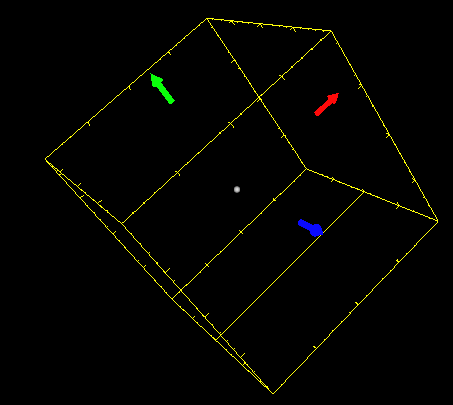
\includegraphics[width=0.3\textwidth]{reference_cube}
	\caption{Reference Cube in Optis}
\end{figure}
}

\longnewglossaryentry{camera-leds}{name=Camera LEDs}{The camera leds (Figure \ref{fig:camera-leds}) are the graphical representation on screen of the real camera leds employed for the movement recording. 
\begin{figure}[h!]
	\centering
	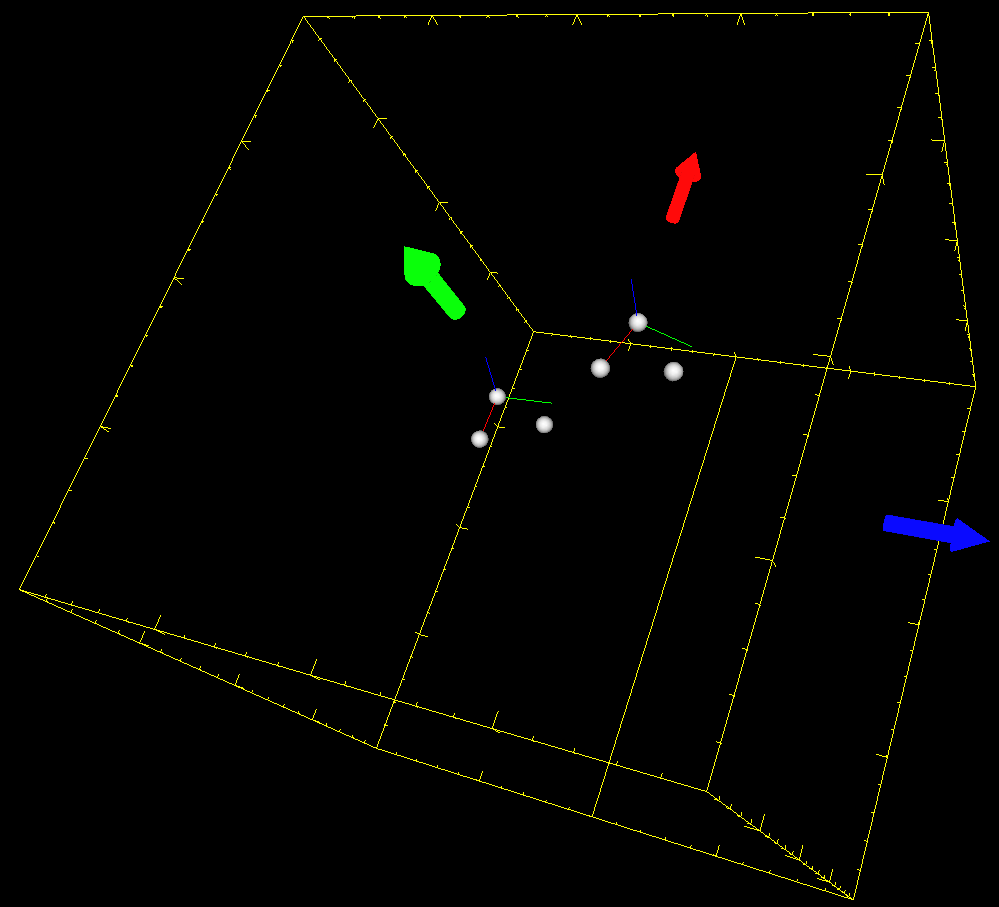
\includegraphics[width=0.4\textwidth]{camera_leds}
	\caption{Camera Leds in \gls{optis}}
	\label{fig:camera-leds}
\end{figure} }

\longnewglossaryentry{optis}{name=Optis}{Proprietary software of the Clinic of Masticatory Disorders used to record in real time the jaw movement of the patient. }

\longnewglossaryentry{tmjviewer}{name=TMJViewer}{Proprietary software of the Clinic of Masticatory Disorders used to display the jaw movement of the patient together with its \glspl{anatomy}. }

\longnewglossaryentry{frame}{name=Frame}{ Almost equivalent to the definition of a film frame. In the \emph{Jaw Viewer} (Listing \ref{code:frame}), a frame contains the data necessary for displaying an object in an exact position in an exact point in time. Like in a movie, several frames build the illusion of movement.}

